\section{Introduction}
\label{sec:intro}

The main purpose of room layout estimation is to extract semantic boundaries among walls, ceiling and floor from a single image. It can be realized by obtaining corresponding semantic planes, as shown in Fig. \ref{fig:pipeline}. The task is challenging because of complex environmental factors such as illumination variations, viewpoints shift, objects diversity and clutter. Furthermore, distinctive clues like room corners and layout boundaries are often occluded by objects. 


\comments{
\begin{figure}[!ht]
	\centering
	\textsc{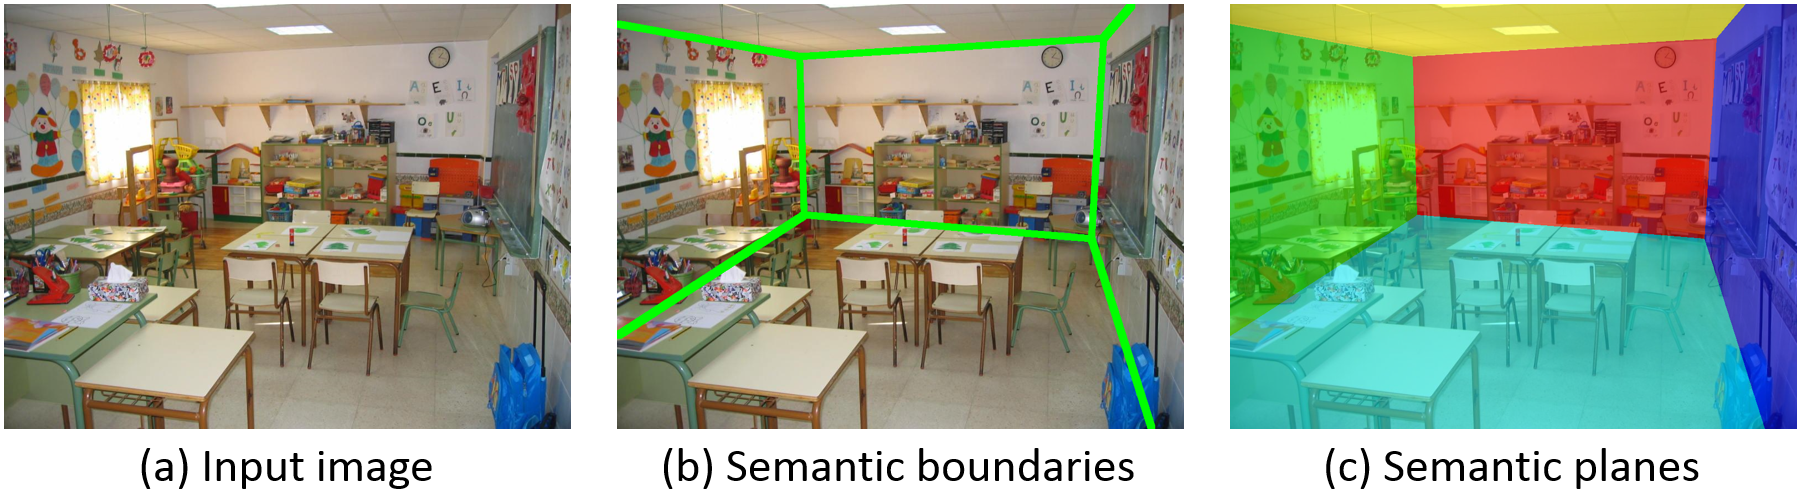
\includegraphics[width=8.5cm]{figure/def.png}}
	\caption{Illustration of the layout estimation problem. (a) Input image. (b) Layout estimation with semantic boundaries. (c) Layout estimation visulized with semantic planes.}
	\label{fig:definition}
\end{figure}
}
\comments{Room layout estimation is a fundamental problem for indoor scene understanding and plays a critical role in a diverse range of applications. For example, scene reconstruction, robot navigation and virtual reality. However, it is challenging that the distinctive clues such as room corners and layout boundaries are often occluded by objects. In addition to the occlusion problem, environmental factors like illumination variations, viewpoints shift, objects diversity and clutter can make the situation worse.}


%%
In recent years, massive researches have been carried out on room layout estimation. Conventional methods usually follow a proposing-ranking framework \cite{hedau2009recovering,wang2013discriminative,gupta2010estimating,hedau2010thinking}. Typically, they first generate numbers of proposals by vanishing point detection and ray sampling. Then a ranking step using hand-crafted features is adopted to select the best hypothesis. Recent methods built on fully convulutional networks (FCNs) or encoder-decoder networks achieve impressive performance \cite{mallya2015learning,ren2016coarse,zhang2016learning,dasgupta2016delay,LeeRoomNet17,zhao2017physics}. Specifically, 
%
Mallya \emph{et al}. \cite{mallya2015learning} presented an FCN for learning informative edge maps from images, which were then integrated into the conventional framework as additional features. 
%
Dasgupta \emph{et al}. \cite{dasgupta2016delay} used an FCN to learn semantic surface labels including \{Left wall, Front wall, Right wall, Ceiling, Ground\} for each pixel. They obtained a segmentation depended on heat maps from FCN and further refined it with geometric projection constraints.
% 
In a subsequent work \cite{ren2016coarse}, Ren \emph{et al}. adopted a multi-task fully convolutional neural network (MFCN) to jointly predict the surface labels and boundaries. Benefit from joint training, the semantic boundaries were more robust and accurate. They also optimized the results later with a refinement framework designed for boundaries.
% 
Zhang \emph{et al}. \cite{zhang2016learning} proposed an another deconvolution network which has multi-layer deconvolution and a receptive field as large as the entire image compared to FCN. As a result, they attained highly reliable edge maps. 
%
End-to-End approach for room layout estimation had been explored by Lee \emph{et al}. \cite{LeeRoomNet17}. They employed an encoder-decoder network to delineate room layout structure using 2D keypoints.
%
Zhao \emph{et al}. \cite{zhao2017physics} introduced a semantic transfer FCN to extract reliable edge features. They fisrt trained an FCN for 37-class semantic segmentation and then bridge the gap to 4-class edge labels by adding a fully connected layer. A physics inspired inference scheme was designed for opimization.


\comments{Typically, the FCNs are trained to segment semantic surfaces or to predict boundaries among them. Followed by a postprocessing scheme, the output from FCNs are refined to be consistent with Fig.~\ref{fig:definition}(b)(c). }

Different from previous FCN based methods, we propose to improve the performance of room layout estimation from another perspective. We consider that global geometric information is as important as texture information in room layout estimation. To implicitly employ the geometric hints, depth and normals are estimated from the original image and fused into an MC-FCN. We use the same formulation of layout in \cite{dasgupta2016delay} and combine their optimization step with a proposing-ranking framework to attain precise layout. Experimental results demonstrate that our method is robust and effective for layout estimation even facing clutter and occlusion.

\comments{
In this paper, we propose to enhance the FCN's ability for room layout estimation by fully utilizing the geometric information of the scene. Our pipeline is shown in Fig.~\ref{fig:pipeline}. First, we estimate depth and normal maps from a single image using network in \cite{eigen2015predicting}. Then we integrate these geometric hints to train a multi-channel FCN for semantic surface segmentation. At last, an extended post-processing algorithm based on \cite{dasgupta2016delay} is applied to generally refine the estimation results. We evaluate our method on two popular benchmark dataset. Experimental results demonstrate that our method is robust and effective for layout estimation even facing clutter and occlusion.
}





